\documentclass [a4paper]{article}
\usepackage{graphicx, amsmath,amssymb,amsfonts}
\usepackage[a4paper, total={8.5in, 13in}, margin=1in]{geometry}
\bibliographystyle{plain}
\usepackage{listings}
\usepackage{xcolor}
\lstset{
    language=Python,
    basicstyle=\ttfamily\small,
    keywordstyle=\color{blue},
    commentstyle=\color{gray},
    stringstyle=\color{red},
    showstringspaces=false,
    frame=single,
    breaklines=true,
    numbers=left,
    numberstyle=\tiny\color{gray},
    tabsize=4,
}

\title{MAT 196 Laboratory Exercise No. 4}
\author{Jeanne Marie B. Quiñanola}
\date{\today}

\begin{document}

\maketitle

\section{Introduction}
In difference equations, the changes in states of a system are modeled over discrete intervals. In most cases, the discrete intervals represent time intervals, and therefore the letter \(t\) is used to denote the time variable.
A form of the difference equation that will be encountered most often is 
\[
x_{t + k} + a_1 x_{t+k-1} + \ldots + a_{k-1} x_{t+1} + a_k x_t = b_t, \quad t = 0, 1,\ldots\]

The order of the difference equation is \(k\), provided \(a_k \neq 0\). The coefficients are assumed to be real and the functions are real-valued. The coefficients \(a_j\), \(j = 1, \ldots, k\), can be functions of \(t\) and state variables \(x_i\) for \(i = t, \ldots, t + k - 1\). The function \(b_t\) on the right-hand side of the equation may depend on \(t\) but not on the state variables.

If the coefficients \(a_j\), \(j = 1, \ldots, k\) in the equation are constant or depend on \(t\) but do not depend on the state variables, then the difference equation is said to be linear. Otherwise, it is said to be nonlinear. In addition, if the difference equation is linear and \(b_t = 0\) for all \(t\), then it is said to be homogeneous; otherwise, it is said to be nonhomogeneous.\cite{linda}

Now, in population dynamics a frequently encountered model for fish population is based on an empirical equation called the Ricker Equation given by 

\[ x_{t + 1} = ax_{t}e^{-bx_{t}},\]

where \(a > 0\) represents the maximal growth rate of fish and \( b > 0 \) is the inhibition of growth caused by overpopulation. \cite{greenwell1984ricker}

For this study, we aim to identify the one-period equilibria of the Ricker equation, analyze the range of parameter values \(a\) and \(b\) for which each equilibrium is either locally asymptotically stable or unstable, and finally, conduct numerical simulations to validate the analytical results.


\section{Analysis and Discussion}

To find the equilibrium of Ricker's equation given by \( x_{t + 1} = ax_{t}e^{-bx_{t}}\), we let: \\

\begin{align*}
f(\bar{x}) &= \bar{x}, \\
a\bar{x}e^{-b\bar{x}} &= \bar{x}\\
a\bar{x}e^{-b\bar{x}} - \bar{x} &= 0\\
\bar{x}(ae^{-b\bar{x}} - 1) &= 0\\
\bar{x_1} &= 0. \\
\end{align*}
To solve for \(\bar{x_2}\) we have: 
\begin{align*}
ae^{-b\bar{x}} - 1 &= 0\\
ae^{-b\bar{x}} &=  1\\
\ln({ae^{-b\bar{x}}}) &= \ln({1})\\
\ln({a}) - b\bar{x} &= 0\\
- b\bar{x} &= -\ln({a})\\
\bar{x_2} &= \frac{\ln({a})}{b}.
\end{align*}

Now, \(\bar{x}\) is locally asymptotically stable if \(| f'(\bar{x})| < 1\) and unstable if  
\(| f'(\bar{x})| > 1\) . 

Let:\\

\begin{align*}
    f(x) &= axe^{-bx}\\
    f'(x) &= (ax)(-be^{-bx}) + (e^{-bx})(a)\\
    &= ae^{-bx}(1-bx).
\end{align*}

Thus, \(\bar{x_1} = 0\) is locally asymptotically stable if: 

\begin{align*}
    f'(\bar{x_1}) &= |ae^{-b(0)}(1-b(0))|\\
    &= |a|\\
    &= a < 1.
\end{align*}

Since Ricker's model only consider \(a > 0\), \(\bar{x_1}\) is locally asymptotically stable if \(0< a < 1\). 

Meanwhile, it is unstable if: \\

\begin{align*}
| f'(\bar{x})| > 1\\
|a| > 1\\
a > 1.
\end{align*}

Now, \(\bar{x_2} = \frac{\ln({a})}{b}\) is locally asymptotically stable if:

\begin{align*}
    f'(\bar{x_2}) &= \left| ae^{-b\left(\frac{\ln(a)}{b}\right)} \left(1 - b\left(\frac{\ln(a)}{b}\right)\right) \right| \\
    &= \left| 1 - \ln(a) \right| < 1.
\end{align*}

\begin{align*}
    \left| 1 - \ln(a) \right| < 1 &\leftrightarrow 
    -1 < 1 - \ln(a) < 1, \\
    &\leftrightarrow -2 < -\ln(a) < 0, \\
    &\leftrightarrow 0 < \ln(a) < 2, \\
    &\leftrightarrow e^0 < a < e^2, \\
    &\leftrightarrow 1 < a < 7.38906.
\end{align*}

Meanwhile, it is unstable if:
\begin{align*}
    \left| 1 - \ln(a) \right| > 1 &\leftrightarrow 
    1 - \ln(a) < -1 \ \text{or} \ 1 - \ln(a) > 1, \\
    &\leftrightarrow \ln(a) > 2 \ \text{or} \ \ln(a) < 0, \\
    &\leftrightarrow a > e^2 \ \text{or} \ a < e^0, \\
    &\leftrightarrow a > 7.38906 \ \text{or} \ a < 1.
\end{align*}
\newpage
\section{Numerical Simulations}
As shown below:

\begin{itemize}
    \item \textbf{Case 1:} \( a = 1.5, \, b = 1.5 \) \\
    We can see that the solution eventually stabilizes at 
    \[
    \bar{x_2} = \frac{\ln(1.5)}{1.5} \approx 0.27031.
    \]

    \item \textbf{Case 2:} \( a = 4.5, \, b = 1.5 \) \\
    We can see that the solution eventually stabilizes at 
    \[
    \bar{x_2} = \frac{\ln(4.5)}{1.5} \approx 1.00272.
    \]

    \item \textbf{Case 3:} \( a = 6.5, \, b = 1.5 \) \\
    We can see that the solution eventually stabilizes at 
    \[
    \bar{x_2} = \frac{\ln(6.5)}{1.5} \approx 1.24787.
    \]

    \item \textbf{Cases 4 and 5:} \\
    Since the values of \( a > 7.38906 \), the equation becomes unstable.
\end{itemize}

The analytical results obtained is consistent with the numerical simulation in Python.
\begin{figure}[h] 
    \centering 
    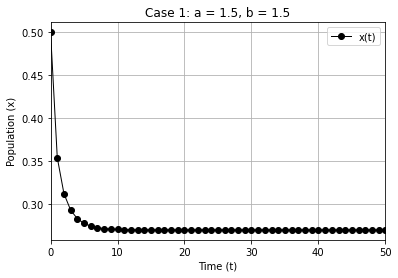
\includegraphics[width=0.80\textwidth]{Fig 1.png} 
\end{figure}
\newpage
\begin{figure}[h]
    \centering 
    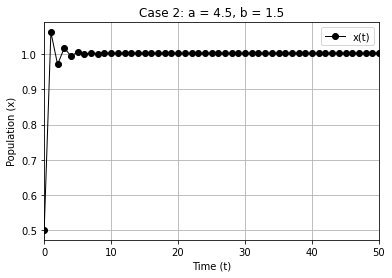
\includegraphics[width=0.80\textwidth]{Fig 2.png} 
\end{figure}
\begin{figure}[h] 
    \centering 
    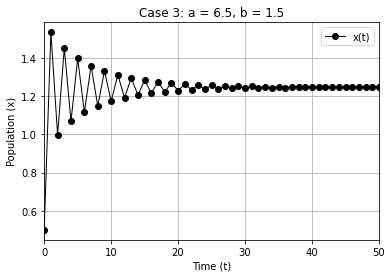
\includegraphics[width=0.80\textwidth]{Fig 3.png} 
\end{figure}
\newpage
\begin{figure}[h]
    \centering 
    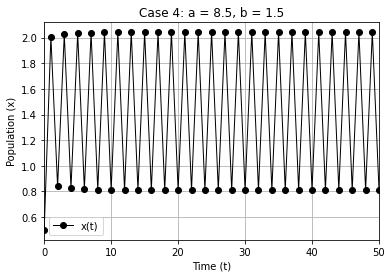
\includegraphics[width=0.80\textwidth]{Fig 4.png} 
\end{figure}
\begin{figure}[h] 
    \centering 
    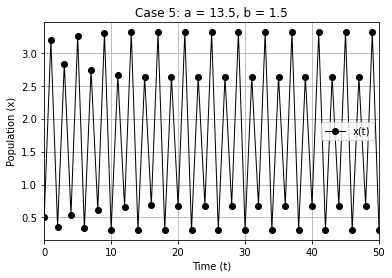
\includegraphics[width=0.80\textwidth]{Fig 5.png} 
\end{figure}
\newpage
\section{Python Code Simulation}

Below is the Python code used for simulating the solution of the Ricker equation.

\begin{lstlisting}[language=Python]
import numpy as np
from numpy import zeros
import matplotlib.pyplot as plt

T = 50
index_set = range(T + 1)
x = zeros(len(index_set))
x[0] = 0.5

# Case 1: a = 1.5, b = 1.5
a = 1.5
b = 1.5

for t in index_set[0:T]:
    x[t + 1] = a * x[t] * np.exp(-b * x[t])

# Plot results
plt.plot(index_set, x, 'ko-', linewidth=1.0, label='x(t)')
plt.xlabel("Time (t)")
plt.ylabel("Population (x)")
plt.title("Case 1: a = 1.5, b = 1.5")
plt.legend(loc="best")
plt.xlim(0, T)
plt.grid()
plt.show()

# Case 2: a = 4.5, b = 1.5
x[0] = 0.5  
a = 4.5
b = 1.5

for t in index_set[0:T]:
    x[t + 1] = a * x[t] * np.exp(-b * x[t])

# Plot results
plt.plot(index_set, x, 'ko-', linewidth=1.0, label='x(t)')
plt.xlabel("Time (t)")
plt.ylabel("Population (x)")
plt.title("Case 2: a = 4.5, b = 1.5")
plt.legend(loc="best")
plt.xlim(0, T)
plt.grid()
plt.show()
\end{lstlisting}

\newpage  

\begin{lstlisting}[language=Python]
# Case 3: a = 6.5, b = 1.5
x[0] = 0.5  
a = 6.5
b = 1.5

for t in index_set[0:T]:
    x[t + 1] = a * x[t] * np.exp(-b * x[t])

# Plot results
plt.plot(index_set, x, 'ko-', linewidth=1.0, label='x(t)')
plt.xlabel("Time (t)")
plt.ylabel("Population (x)")
plt.title("Case 3: a = 6.5, b = 1.5")
plt.legend(loc="best")
plt.xlim(0, T)
plt.grid()
plt.show()

# Case 4: a = 8.5, b = 1.5
x[0] = 0.5  
a = 8.5
b = 1.5

for t in index_set[0:T]:
    x[t + 1] = a * x[t] * np.exp(-b * x[t])

# Plot results
plt.plot(index_set, x, 'ko-', linewidth=1.0, label='x(t)')
plt.xlabel("Time (t)")
plt.ylabel("Population (x)")
plt.title("Case 4: a = 8.5, b = 1.5")
plt.legend(loc="best")
plt.xlim(0, T)
plt.grid()
plt.show()

# Case 5: a = 13.5, b = 1.5
x[0] = 0.5  
a = 13.5
b = 1.5

for t in index_set[0:T]:
    x[t + 1] = a * x[t] * np.exp(-b * x[t])

# Plot results
plt.plot(index_set, x, 'ko-', linewidth=1.0, label='x(t)')
plt.xlabel("Time (t)")
plt.ylabel("Population (x)")
plt.title("Case 5: a = 13.5, b = 1.5")
plt.legend(loc="best")
plt.xlim(0, T)
plt.grid()
plt.show()
\end{lstlisting}
\newpage
\section{Summary and Conclusions}

In this paper, we analyzed a mathematical model known as Ricker equation, which is widely used to model fish populations. We derived and solved for its equilibria, identifying \( x_1 = 0 \) and \( x_2 = \frac{\ln(a)}{b} \) as the equilibrium points of the system. Furthermore, we determined the conditions under which these equilibria are locally asymptotically stable or unstable.

Specifically, we found that \( x_2 \) is stable when \( 1 < a < 7.38906 \) and becomes unstable when \( a > 7.38906 \).

To validate these findings, we performed numerical simulations for different values of \( a \) and \( b \). The results confirmed our analytical predictions, demonstrating consistency between theory and simulation. For instance:
\begin{itemize}
    \item For \( a = 1.5, b = 1.5 \), the solution stabilized at \( x_2 = \frac{\ln(1.5)}{1.5} \approx 0.27031 \).
    \item For \( a = 4.5, b = 1.5 \), the solution stabilized at \( x_2 = \frac{\ln(4.5)}{1.5} \approx 1.00272 \).
    \item For \( a = 6.5, b = 1.5 \), the solution stabilized at \( x_2 = \frac{\ln(6.5)}{1.5} \approx 1.24787 \).
    \item For \( a > 7.38906 \), the equation became unstable as predicted by our analysis.
\end{itemize}
These findings highlight the importance of parameter selection in ensuring stable population dynamics in models like Ricker equation. 
\bibliography{citation} 
\end{document}
 